\chapter{Technical Foundation}
\label{cha:technical-foundation}

This chapter will give an overview of the technical knowledge required for this thesis. It will give an exposure to the different type systems, the programming language JavaScript and JavaScript supersets. Also the terminology used throughout this paper will be specified, since standard terminology differs across sources~\cite[p.~1]{TypeSystems:Cardelli:2004}.

\section{Type Systems}
\label{sec:type-systems}

There are different kinds of programming languages with different characteristics and specifications. An essential part of a language is its type system, which has a great impact on the behavior of a program and may influence the syntax the program is written in.
In general a programming language can be categorized as typed or untyped, where untyped languages do not have a static type system at all, or have a single type that can hold any value~\cite[p.~2]{TypeSystems:Cardelli:2004}. More precisely a language is considered typed independently of types being part of the syntax, but simply by the existence of a (static) type system~\cite[p.~2]{TypeSystems:Cardelli:2004}.
According to \citeauthor{TypeSystems:Cardelli:2004} from \emph{Microsoft Research\footnote{https://www.microsoft.com/research/}} a type system is
\begin{quote}
  [a] collection of type rules for a typed programming language~\cite[p.~38]{TypeSystems:Cardelli:2004}
\end{quote}
with the purpose to
\begin{quote}
  [...] prevent the occurrence of \emph{execution errors} during the running of a program~\cite[p.~1]{TypeSystems:Cardelli:2004}.
\end{quote}
He further equates \emph{type system} with \emph{static type system} and also \citeauthor{TypesAndProgrammingLanguages:Pierce:2002} defines type systems as being static~\cite[p.~2]{TypesAndProgrammingLanguages:Pierce:2002}, which categorizes languages as untyped, that may distinguish between types in run time, but do not have knowledge about types during compile time or interpretation, such as JavaScript (see section~\ref{sec:language-introduction}). This notion is further supported by \citeauthor{ProgrammingLanguagesPrinciplesAndPractices:LoudenLambert:2011}, stating that
\begin{quote}
  [l]anguages without static type systems are usually called untyped languages (or dynamically typed languages). Such languages include [...] most scripting languages such as Perl, Python, and Ruby~\cite[p.~331]{ProgrammingLanguagesPrinciplesAndPractices:LoudenLambert:2011}.
\end{quote}
Obviously, a widely adopted consensus in terminology is to use both, \emph{untyped} (e.g.\ in~\cite[p.~117]{LogicalTypesForUntypedLanguages:Tobin-Hochstadt:2010}) and \emph{dynamically typed} (e.g.\ in~\cite[p.~32]{TowardsAProgramLogicForJavaScript:Gardner:2012} and~\cite[p.~203]{TypeSystemsDirectedProgrammingLanguageEvolution:Nino:2012}) for languages without a static type system. Anyway, following the terminology of \citeauthor{TypeSystems:Cardelli:2004}, expressions like \emph{statically typed} or \emph{dynamically typed} are avoided in favor for \emph{statically checked} and \emph{dynamically checked}, respectively~\cite[p.~1]{TypeSystems:Cardelli:2004}. This should help to avoid confusion over languages having types, but are referred to as untyped.

% While a type system may help in preventing execution errors, a programming language is not required to have a type system to ensure against specific errors, as there are mechanisms for untyped languages to make them safe. % runtime type checks (see ..!)

\subsection{Explicitly and Implicitly Typed}
\label{sec:explicitly-implicitly-typed}

If types are part of the syntax of a language (e.g.\ Java) it is explicitly typed, whereas in implicitly typed languages, type annotations are assigned automatically by the type system~\cite[pp.~2--3]{TypeSystems:Cardelli:2004}. Some languages, however, make use of a mixture, allowing developers to omit type annotations in various scenarios, where the type can be inferred by the compiler~\cite[p.~10]{TypesAndProgrammingLanguages:Pierce:2002} as shown in the C\texttt{\#} code below:
\begin{CsCode}[numbers=none]
var implicitNum = 10; // implicitly typed as integer
int explicitNum = 10; // explicitly typed as integer
\end{CsCode}
While a type system---explicit, implicit or a combination of both---may detect possible execution errors already during compile time, it is not required to guard against specific errors. There are mechanisms for untyped languages to make them safe~\cite[p.~3]{TypeSystems:Cardelli:2004}, as outlined in section~\ref{sec:type-checking}.

\subsection{Execution Errors}
\label{sec:execution-errors}
% runtime
Errors can occur in various situations and in order to classify a language, it is important to understand the different types of errors. \citeauthor{TypeSystems:Cardelli:2004} distinguished between three error categories: Trapped errors, untrapped errors and forbidden errors~\cite[p.~3]{TypeSystems:Cardelli:2004}.

\subsubsection{Trapped Errors}

A trapped error causes a program to stop immediately~\cite[p.~3]{TypeSystems:Cardelli:2004} or to raise an exception, which may be handled in the program~\cite[p.~7]{TypesAndProgrammingLanguages:Pierce:2002}. An example for such an error could be division by zero~\cite[p.~3]{TypeSystems:Cardelli:2004}.

\subsubsection{Untrapped Errors}

Errors where a program does not crash or raise an exception immediately are called untrapped errors~\cite[p.~37]{TypeSystems:Cardelli:2004}. They may remain unnoticed---at least for a while---and can lead to unexpected behavior~\cite[p.~3]{TypeSystems:Cardelli:2004}. For example accessing data from an array that is out of bounds is perfectly legal in the programming language C~\cite[p.~7]{TypesAndProgrammingLanguages:Pierce:2002}, but can lead to errors or arbitrary behavior later in the program~\cite[p.~3]{TypeSystems:Cardelli:2004}.

\subsubsection{Forbidden Errors}

Following the definition of \citeauthor{TypeSystems:Cardelli:2004}, forbidden errors should include ``all of the untrapped errors, plus a subset of the trapped errors~\cite[p.~3]{TypeSystems:Cardelli:2004}''. They are not generally defined, but vary between programming languages and may even not include all untrapped errors, which leads to a language being  considered as unsafe~\cite[p.~4]{TypeSystems:Cardelli:2004}.

% sound
\subsection{Safety and Good Behavior}
\label{sec:safety-good-behavior}

A programming language can be considered as safe if no untrapped errors can appear, and is well behaved (i.e., good behaved), if no forbidden errors can occur~\cite[p.~3]{TypeSystems:Cardelli:2004}, consequently good behavior implies safety. Not all major languages are safe, and therefore not well behaved, such as C or C\texttt{++}~\cite[p.~6]{TypesAndProgrammingLanguages:Pierce:2002}, as guaranteeing safety usually results in increased execution time. An example for a safe language, with decreased development and maintenance time compared to an unsafe language, is Java~\cite[p.~5]{TypeSystems:Cardelli:2004}.

\subsection{Type Checking}
\label{sec:type-checking}

To ensure that a program follows the specified rules of its type system and to guarantee safety and good behavior (i.e., ensuring the absence of forbidden errors~\cite[p.~37]{TypeSystems:Cardelli:2004}), as described in section~\ref{sec:safety-good-behavior}, type checking may be performed. Again, \citeauthor{TypeSystems:Cardelli:2004} treats \emph{type checking} and \emph{static type checking} as equivalent and calls languages that employ such a technique \emph{statically checked}~\cite[p.~3]{TypeSystems:Cardelli:2004}. Dynamically checked programming languages, on the other hand, may also ensure good behavior by applying sufficient checks at run time. Anyway, statically checked languages may also perform checks during the execution of a program to guarantee safety, if not all untrapped errors can be discovered statically during compilation~\cite[p.~4]{TypeSystems:Cardelli:2004}.

%\subsubsection{Static Checking}
%
%\subsubsection{Dynamic Checking}

% How safety is accomplished can differ,

%\begin{itemize}
%\item Trapped Error
%\item Untrapped Error
%\item Forbidden Error
%\end{itemize}

% Strongly Checked, Weakly Chechecked

% Terminology; Soundness and Safety; Strongly and Weekly Checked, Well Typed and Well Behaved

%\subsection{Explicit and Implicit Typing}
%\label{sec:explicit-implicit-typing}

%Explicitly typed languages require a programmer to define types manually in a program as shown below.
%\begin{JavaCode}[numbers=none]
%int i = 10;
%boolean b = true;
%\end{JavaCode}
%Languages that are typed implicitly may look like the following:
%\begin{JsCode}[numbers=none]
%let i = 10;
%let b = true;
%\end{JsCode}

%\subsection{Static and Dynamic Typing}
%\label{sec:static-dynamic-typing}
%
%\subsection{Strong and Weak Typing}
%\label{sec:strong-weak-typing}

% In strongly typed languages it is guaranteed that there will be no forbidden errors at run time, where in weakly typed languages such errors may occur~\cite[p.~97-38]{ComputerScienceHandbook}. 

\section{JavaScript}
\label{sec:javascript}

JavaScript dates back to 1996, where its creator Brendan Eich from the company \emph{Netscape\footnote{\emph{Netscape Communications}---founded as \emph{Mosaic} in 1994---released its \emph{Netscape Communicator} browser in 1995 which became the leading internet browser at that time~\cite{HistoryOfNetscape:Cooper:2014}.}} submitted the language to Ecma International\footnote{https://www.ecma-international.org}~\cite[p.~28]{ProJavaScriptDevelopment:Odell:2014}, an ``industry association founded in 1961, dedicated to the standardization of information and communication systems~\cite{EcmaInternational:Ecma}'' and since became one of the most popular programming languages in the world~\cite[p.~2]{JavaScriptTheGoodParts:Crockford:2008}. According to \emph{GitHub\footnote{https://github.com}} it was the most popular language on its platform by opened \emph{Pull Requests\footnote{Pull requests on GitHub are used to let other people know about changes made to a repository. From there on these modification can be reviewed and discussed with collaborators and can be rejected or merged into the repository~\cite{GitHubPullRequest:GitHub:2014}.}} with a growth of 97\% in 2016, followed by Java, which saw an increase of 63\% compared to 2015. Also \emph{TypeScript} (see \ref{sec:typescript}) is following up, which takes the 15th place with an increase of Pull Request by 250\%~\cite{GitHubOctoverse2016:GitHub:2016}.

While JavaScript is known for programming inside browsers and adding visual effects to websites~\cite[p.~4]{JavaScriptObjectProgramming:Rinehart:2015}, its first use in a product was on the server-side in 1994~\cite[p.~369]{ProJavaScriptDevelopment:Odell:2014}. Since then, no application platform for JavaScript was available for 17 years until Ryan Dahl created and released \emph{Node.js\footnote{https://nodejs.org}} in 2011, which allowed developers to build cross-platform applications in JavaScript. It is built upon Google`s \emph{V8 JavaScript engine}, also used in the popular \emph{Chrome\footnote{https://www.google.com/chrome/}} browser~\cite[p.~369]{ProJavaScriptDevelopment:Odell:2014}.

% Add info about ECMAScript? JS and ES used as synonyms for the most parts. ES to distinguish versions/editions

The following sections try to give an ample exposure to the language JavaScript, outlining its most important and interesting concepts. Please note, that not all cases---especially the numerous exceptions---are described, as this would go beyond the scope of this thesis.

\subsection{Loose Typing}
\label{sec:untyped-loosely-typed}

Like in other programming languages, variables can be declared and values may be assigned to them. An essential concept of JavaScript is its loose typing, meaning that any value may be assigned or reassigned at any time to any variable:
\begin{JsCode}[numbers=none]
let foo = 10;
foo = "I've been a number, now I'm a string";
\end{JsCode}
The term \emph{loose typing} may be misleading to infer that JavaScript has a type system. However, when following standard terminology and keeping in mind that type system is equal to \emph{static} type system, it is made clear, that JavaScript is considered untyped. It does employ mechanisms to reject code from running, that has semantic errors, but evaluation is performed during execution, and errors are determined and reported during run time~\cite[p.~291]{ES6Spec:Ecma:2015}. Therefore JavaScript can be deemed a \emph{dynamically checked} language (see section~\ref{sec:type-checking}).

\subsection{Value Types}
\label{sec:value-types}

JavaScript is an untyped and dynamically checked---but safe---scripting language, as defined in section~\ref{sec:type-systems}. Most untyped programming languages are necessarily safe, as it would be exceedingly difficult to maintain the code if untrapped errors would remain unnoticed~\cite[p.~4]{TypeSystems:Cardelli:2004}. Even though considered as untyped, the EcmaScript language specification defines seven value types~\cite[p.~16]{ES6Spec:Ecma:2015}:
\begin{itemize}
  \item Undefined
  \item Null
  \item Boolean
  \item String
  \item Symbol
  \item Number
  \item Object
\end{itemize}
A major difference to a (statically) typed language is, that in JavaScript only values are typed, variables are not. When requesting the type of a variable with the \texttt{typeof} operator during run time, the assigned value's type is determined and returned as a string~\cite[p.~30]{YDKJS:UpAndGoing:Simpson:2015}:
\begin{JsCode}[numbers=none]
let num = 10;
typeof num; // "number"
\end{JsCode}
The returned string by \texttt{typeof} does not reflect the specified value types entirely. As shown in table~\ref{tab:typeof}, objects are differentiated by wether they are callable or not. For objects with a call signature \texttt{"function"} will be returned and \texttt{"object"} otherwise. Strangely, for a value of type \emph{Null}, the result will be \texttt{"object"}. A proposal to change the specification and to fix this bug---erroneously indicating that null is an object---was rejected, as existing code may break~\cite{TypeofNull:Smith:2013, typeof:MDN:2017}.

\begin{table}
\caption{Result of the \texttt{typeof} operator by a value's type~\cite[p.~164]{ES6Spec:Ecma:2015}.}\label{tab:typeof}
\centering
  \setlength{\tabcolsep}{5mm} % separator between columns
  \def\arraystretch{1.25} % vertical stretch factor
  \begin{tabular}{|c|c|}
    \hline
    \emph{Type of Value} & \emph{Result} \\
    \hline \hline
    Undefined & \texttt{"undefined"} \\
    \hline
    Null & \texttt{"object"} \\
    \hline
    Number & \texttt{"number"} \\
    \hline
    String & \texttt{"string"} \\
    \hline
    Symbol & \texttt{"symbol"} \\
    \hline
    Object (not callable) & \texttt{"object"} \\
    \hline
    Object (callable) & \texttt{"function"} \\
    \hline
  \end{tabular}
\end{table}

\subsection{Type Conversion}
\label{sec:type-conversion}

In JavaScript ``any [...] value can be converted to a boolean value~\cite[p.~40]{JavaScriptTheDefinitiveGuide:Flanagan:2011}''. If the interpreter expects a boolean value, it simply performs a conversion~\cite[p.~46]{JavaScriptTheDefinitiveGuide:Flanagan:2011} (see section~\ref{sec:value-conversion}). Because of that it is important to know, which values are considered true, and which conversion will result in being false, depending on their type, as shown in table~\ref{tab:truthy-falsy}.
\begin{table}
\caption{Values evaluated as false or true when converted to a boolean value~\cite[p.~40]{JavaScriptTheDefinitiveGuide:Flanagan:2011}.}\label{tab:truthy-falsy}
\centering
  \def\rr{\rightskip=0pt plus1em \spaceskip=.3333em \xspaceskip=.5em\relax}
  \setlength{\tabcolsep}{1ex}
  \def\arraystretch{1.20}
  \setlength{\tabcolsep}{1ex}
  \begin{tabular}{|c||l|}
    \hline
    \emph{Falsy} & \texttt{undefined}, \texttt{null}, \texttt{0}, \texttt{-0}, \texttt{NaN} and \texttt{""}~(empty string). \\
    \hline
    \emph{Truthy} & {\rr Any other value, including \texttt{[]}~(empty array) and \texttt{\{\}}~(empty object). } \\
    \hline
  \end{tabular}
\end{table}
There are various situation where a conversion is desired, which happens implicitly in JavaScript. For example if a string should be added to a number, and vice versa, the number is converted to a string and the result is a concatenation of both values:
\begin{JsCode}[numbers=none]
"2" + 3 // "23"
"Hello" + 2 + 3 // "Hello23"
\end{JsCode}
The outcome of such an operation will most likely complete without errors, as the interpreter does its best to come up with a sufficient result. Anyway, it has a major influence on the result, how such an expression is written. In the example above, the string was seen first by JavaScript, therefore the subsequent numbers were converted to a string. If, on the other hand, the numbers came first, the result would have been completely different:
\begin{JsCode}[numbers=none]
2 + 3 + "Hello" // "5Hello"
\end{JsCode}
Again, even a slight change to the code means an entirely different outcome:
\begin{JsCode}[numbers=none]
"2" + 3 + "Hello" // "23Hello"
\end{JsCode}
A more comprehensive overview of possible type conversions, summarized by \citeauthor{JavaScriptTheDefinitiveGuide:Flanagan:2011} and extended with Symbol type conversions as of the latest ECMAScript 2015 specification, can be found in table~\ref{tab:conversions}, which also highlights situations, where type conversions are not possible or lead to an error.

% Although conversion between types is performed by JavaScript, it is possible to explicitly perform a cast. (Explicit conversion)

\begin{table}
\caption{Type conversions in JavaScript~\cites[p.~46]{JavaScriptTheDefinitiveGuide:Flanagan:2011}[pp.~36--44]{ES6Spec:Ecma:2015}.}\label{tab:conversions}
\centering
  \def\rr{\rightskip=0pt plus1em \spaceskip=.3333em \xspaceskip=.5em\relax}
  \setlength{\tabcolsep}{1ex}
  \def\arraystretch{1.20}
  \setlength{\tabcolsep}{1ex}
  \small
  \begin{threeparttable}
  \begin{tabular}{|l||c|c|c|c|c|} % p{0.25\textwidth}
    \hline
      \multicolumn{1}{|c}{\emph{Initial Value}} &
      \multicolumn{1}{|c}{\emph{String}} &
      \multicolumn{1}{|c}{\emph{Number}} &
      \multicolumn{1}{|c|}{\emph{Boolean}} &
      \multicolumn{1}{|c|}{\emph{Object}} \\
    \hline\hline
      \texttt{undefined} &
      \texttt{"undefined"} &
      \texttt{NaN} &
      \texttt{false} &
      \emph{TypeError} \\
    \hline
      \texttt{null} &
      \texttt{"null"} &
      \texttt{0} &
      \texttt{false} &
      \emph{TypeError} \\
    \hline\hline
      \texttt{true} &
      \texttt{"true"} &
      \texttt{1} & &
      \footnotesize(\romannum{1}) \\
    \hline
      \texttt{false} &
      \texttt{"false"} &
      \texttt{0} &
      &
      \footnotesize(\romannum{1}) \\
    \hline\hline
      \texttt{""} (empty string) &
      &
      \texttt{0} &
      \texttt{false} &
      \footnotesize(\romannum{1}) \\
    \hline
      \texttt{"1.2"} (non-empty, numeric) &
      &
      \texttt{1.2} &
      \texttt{true} &
      \footnotesize(\romannum{1}) \\
    \hline
      \texttt{"one"} (non-empty, non-numeric) &
      &
      \texttt{NaN} &
      \texttt{true} &
      \footnotesize(\romannum{1}) \\
    \hline\hline
      \texttt{0} &
      \texttt{"0"} &
      &
      \texttt{false} &
      \footnotesize(\romannum{1}) \\
    \hline
      \texttt{-0} &
      \texttt{"0"} &
      &
      \texttt{false} &
      \footnotesize(\romannum{1}) \\
    \hline
      \texttt{NaN} &
      \texttt{"NaN"} &
      &
      \texttt{false} &
      \footnotesize(\romannum{1}) \\
    \hline
      \texttt{Infinity} & 
      \texttt{"Infinity"} &
      &
      \texttt{true} &
      \footnotesize(\romannum{1}) \\
    \hline
      \texttt{-Infinity} &
      \texttt{"-Infinity"} &
      &
      \texttt{true} &
      \footnotesize(\romannum{1}) \\
    \hline
      \texttt{1} (finite, non-zero) &
      \texttt{"1"} &
      &
      \texttt{true} &
      \footnotesize(\romannum{1}) \\
    \hline\hline
      \texttt{\{\}} (any object) &
      \footnotesize(\romannum{2}) &
      \footnotesize(\romannum{3}) &
      \texttt{true} &
      \\
    \hline
      \texttt{[]} (empty array) &
      \texttt{""} &
      \texttt{0} &
      \texttt{true} &
      \\
    \hline
      \texttt{[9]} (single numeric array) &
      \texttt{"9"} &
      \texttt{9} &
      \texttt{true} &
      \\
    \hline
      \texttt{["a"]} (any other array) &
      \footnotesize(\romannum{4}) &
      \texttt{NaN} &
      \texttt{true} &
      \\
    \hline
      \texttt{() => \{\}} (any function) &
      \footnotesize(\romannum{2}) &
      \texttt{NaN} &
      \texttt{true} &
      \\
    \hline
      \texttt{Symbol("sym")} (any symbol) &
      \emph{TypeError} &
      \emph{TypeError} &
      \texttt{true} &
      \footnotesize(\romannum{1}) \\
    \hline
  \end{tabular}
  \begin{tablenotes}
    \footnotesize
    \item (\romannum{1}) For situations, where converting a value to an object does not throw a TypeError, a new object of the value's type is returned. E.g.\ for the value \texttt{"Hello world!"}, \texttt{new String("Hello world!")} is returned~\cite[p.~44]{ES6Spec:Ecma:2015}.
    \item \footnotesize(\romannum{2}) When converting an object to a string, JavaScript tries to call the \texttt{toString} or \texttt{valueOf} method on the object and converts the returned value to a string. If no primitive value can be obtained from either of these methods, a TypeError is thrown~\cite[p.~50]{JavaScriptTheDefinitiveGuide:Flanagan:2011}.
    \item \footnotesize(\romannum{3}) The same steps as in \footnotesize(\romannum{2}) are performed with the difference, that \texttt{valueOf} will be preferred over \texttt{toString}.
    \item \footnotesize(\romannum{4}) The toString method of the Array object joins the array separated by a comma, which would result in \texttt{["a","b","c"]} being converted to \texttt{"a,b,c"}~\cite{ArrayPrototypeToString:MDN:2017}.
  \end{tablenotes}
\end{threeparttable}
\end{table}

%When taking a look at table~\ref{tab:truthy-falsy}, the following examples are considered equal and evaluate to true:
%\begin{JsCode}
%"" == false
%
%\end{JsCode}
%whereas the expressions below will be false:
%\begin{JsCode}
%"" == true
%null == -1
%1 == NaN
%!1
%{} == ""
%\end{JsCode}
%In order to check if a value \emph{and} type of compared values actually equals, without performing a conversion, the strict equality operator may be used as such:
%\begin{JsCode}
%"1" === "1" // true
%"1" === 1 // false
%\end{JsCode}

\subsection{Value Comparison}
\label{sec:value-conversion}

In section~\ref{sec:value-conversion}, the flexibility of JavaScript has already been outlined. Types are converted (i.e., casted) to another type if required and possible.  The same is true when comparing values. JavaScript tries to implicitly convert a value to another type if it cannot perform a comparison at first. Comparing a string---holding a numerical value---with an actual number, will give the same result as comparing two values of type Number, as the interpreter implicitly casts the string to a number:
\begin{JsCode}[numbers=none]
"5" > 2 // true
"2" == 2 // true
\end{JsCode}
When comparing with the \emph{equality operator} \texttt{==} there are a few rules to keep in mind~\cite[~p.~72]{JavaScriptTheDefinitiveGuide:Flanagan:2011}:
\begin{itemize}
  \item The values \texttt{null} and \texttt{undefined} are considered equal.
  \item If a number and a string are compared, the string is converted to a number.
  \item The values \texttt{true} and \texttt{false} are converted to \texttt{1} and \texttt{0} respectively.
  \item Objects are compared by reference\footnote{Todo: Explain by reference and by value shortly}, whereas one value being a number and the other one being a string, JavaScript tries to convert it to a primitive value, either by using the object's toString or valueOf method.
  \item All other comparisons are not equal.
\end{itemize}
If a more strict comparison is required and an automatic conversion of values is not desired, the \emph{strict equality operator} \texttt{===} may be used. Only if type and value matches, the expression evaluates to true:
\begin{JsCode}[numbers=none]
"2" === 2 // false
2 === 2   // true
\end{JsCode}
Following the rules from above it is interesting to look at comparing an object to the string \texttt{[object Object]}:
\begin{JsCode}[numbers=none]
{} == "[object Object]"  // true
{} === "[object Object]" // false
\end{JsCode}
Using the equality operator, the object is converted using the default toString method, returning \texttt{"[object Object]"}, resulting in the compared values being equal. When making use of the \emph{strict} equality operator, no conversion is performed and the expression is false.

% {} == "[object Object]" // true
% {} === "[object Object]" // false

% NaN never true

%At this point it is important to keep the values considered as truthy or falsy from table~\ref{tab:truthy-falsy} in mind. 
%Checking for equality on two truthy or falsy values evaluates to true:
%\begin{JsCode}[numbers=none]
%0 == "" // true
%\end{JsCode}
%Besides JavaScript converting values if necessary, it does not perform a cast, if the types of the values match. E.g.\ comparing \texttt{NaN} to \texttt{0}, will evaluate to \texttt{false}. Both values are of type Number. 
%In order to check if a value's type actually equals a type, the strict equality operator may be used as such:
%\begin{JsCode}
%"1" === 1   // false
%"1" === "1" // true
%\end{JsCode}



% The flexibility of JavaScript 

% NaN

\subsection{Objects and Prototypal Inheritance}
\label{sec:objects-prototypal-inheritance}

Every value that is not a primitive value (i.e., Undefined, Null, Boolean, Number, Symbol, or String~\cite[p.~5]{ES6Spec:Ecma:2015})---including functions and arrays---is an object, hence making JavaScript a highly flexible language. A key concept of the language is the prototypal inheritance of objects. Every object has a prototype, which is just a reference to another object. Anyway, the prototype is not accessible for all types of objects, but for functions, or more precisely, constructors~\cite[p.~3]{ES6Spec:Ecma:2015} (see figure~\ref{fig:prototypal-inheritance}).
A constructor function is just an ordinary JavaScript function, that---by convention---begins with a capital letter~\cite[p.~8]{JavaScriptObjectProgramming:Rinehart:2015}. Initial values can be defined, that may be different for every instance created from the constructor.
\begin{JsCode}[numbers=none]
function Person(name) {
  this.name = name;
}
\end{JsCode}
On the other hand, properties on the function's prototype may be defined. This properties are shared across all instances of \emph{Person}.
\begin{JsCode}[numbers=none]
Person.prototype.speak = function speak() {
  return "Hi, my name is " + this.name;
}
\end{JsCode}
By calling \texttt{thomas.speak()} in the code below, JavaScript looks for a \emph{speak} property on the object \emph{thomas}. As there doesn't exist any property with that name, the interpreter looks at the object's prototype and successfully calls the method~\cite[pp.~85--86]{YDKJS:ThisAndObjectPrototypes:Simpson:2015}.
\begin{JsCode}[numbers=none]
let thomas = new Person("Thomas");
thomas.speak(); // "Hi, my name is Thomas"
\end{JsCode}
If again no property \emph{speak} would exist on the prototype, JavaScript would look at the prototype's prototype, and so on. This is called the prototype chain~\cite[p.~86]{YDKJS:ThisAndObjectPrototypes:Simpson:2015}.

\begin{figure}
\centering
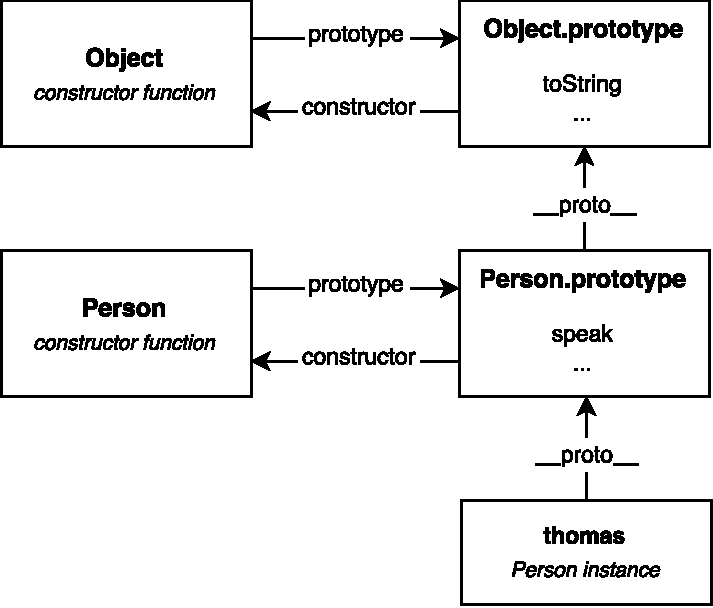
\includegraphics[width=.65\textwidth]{prototypal-inheritance}
\caption{Prototypal inheritance in JavaScript.}
\label{fig:prototypal-inheritance}
\end{figure}

\subsection{Latest Improvements}

JavaScript is recently improving rapidly, with a number of minor and major additions and improvements to the language's standard. Some additions improve readability and reduce the amount of lines of code needed to accomplish the same things in previous versions. Others add completely new functionality and concepts to JavaScript. The following few sections will give a shallow overview of a few additions to the 6th edition of ECMAScript---called \emph{ECMAScript 2015}---as they make it most distinctive to the standard's previous edition.

\label{sec:latest-improvements}

\subsubsection{Declaration Keywords}

Until and including the fifth edition of ECMAScript (i.e., ES5), the only declaration keyword available was \texttt{var}~\cite[p.~87]{ES5Spec:Ecma:2015}. As of the sixth edition of ECMAScript (i.e., ES6), the keywords \texttt{let}---as seen in previous code snippets---and \texttt{const} were added~\cite[p.~194]{ES6Spec:Ecma:2015}. In order to understand the impact of using one keyword over another, it is important to know the basics of how variables are scoped in JavaScript. \citeauthor{YDKJS:ScopesAndClosures:Simpson:2014} defines a scope as 
\begin{quote}
  [...] the set of rules that govern how the engine can look up a variable by its identifier name and find it, either in the current scope, or in any of the nested scopes it’s contained within~\cite[p.~13]{YDKJS:ScopesAndClosures:Simpson:2014}.
\end{quote}
JavaScript makes use of a \emph{lexical scope} model, which is based on where variables and scope blocks (e.g. functions) are written in the code~\cite[p.~13]{YDKJS:ScopesAndClosures:Simpson:2014}. This means that 
\begin{quote}
  [n]o matter \emph{where} a function is invoked from, or even \emph{how} it is invoked, its lexical scope is \emph{only} defined by where the function was declared~\cite[p.~16]{YDKJS:ScopesAndClosures:Simpson:2014}.
\end{quote}
Program~\ref{prog:scopes} gives a simple example of how scopes behave in JavaScript and also shows the importance to be aware of it. While there are ways to get around lexical scoping in JavaScript, those mechanisms are considered bad practice~\cite[p.~14]{YDKJS:ScopesAndClosures:Simpson:2014} and come with performance issues~\cite[p.~21]{YDKJS:ScopesAndClosures:Simpson:2014}, hence won't be covered here.

\begin{program}
\caption{Variable \texttt{i} was declared on line 7 as counter for a for loop. When function \texttt{bar} is called from the loop, the identifier \texttt{i} exists in the scope of \texttt{bar}, or rather in its enclosing scope \texttt{foo}, and \texttt{i} is assigned the value \texttt{2}. This results in an infinite loop, as the loop will never reach its condition to stop of \texttt{i} being equal to or greater than \texttt{10}.~\cite[p.~26]{YDKJS:ScopesAndClosures:Simpson:2014}}
\label{prog:scopes}
\begin{JsCode}
function foo() {

  function bar() {
    i = 2;
  }
  
  for(var i = 0; i < 10; i++) {
    bar();
  }
  
}

foo();
\end{JsCode}
\end{program}

Before \texttt{let} and \texttt{const} were introduced, the easiest way to create a scope was a function~\cite[p.~7]{YDKJS:ES6AndBeyond:Simpson:2015}. Other programming languages, like Java, support block scope~\cite[p.~7]{YDKJS:ScopesAndClosures:Simpson:2014}, which means that variables will be scoped by any block that is created, including loops. JavaScript, however, has a function scope, as shown previously in program~\ref{prog:scopes}. As of ES6, with \texttt{let} it is possible to make use of block scoped variables, whereas \texttt{var} would lead to the variable being scoped to its parent function or the global scope, if no enclosing function exists. The code below demonstrates, that creating a simple block in JavaScript in combination with a \texttt{var} declaration, does not scope the identifier to that block~\cite[p.~8]{YDKJS:ES6AndBeyond:Simpson:2015}.
\begin{JsCode}
var a = 1;

{
  var a = 2
}

console.log(a); // 2
\end{JsCode}
On the other hand, when declaring \texttt{a} on line 4 with the \texttt{let} keyword, the variable will be scoped to its enclosing block. In this case it doesn't make any difference, whether the declaration on the first line uses \texttt{var} or \texttt{let}, as it is top level and will live in the global scope anyway.
\begin{JsCode}
var a = 1;

{
  let a = 2
}

console.log(a); // 1
\end{JsCode}
Anyway, it may be a good practice to use the block scope behavior for variables with \texttt{let} or \texttt{const} over \texttt{var} at any time, if not explicitly needed otherwise. This may prevent errors and unexpected behavior, as shown in program~\ref{prog:scopes-let}, when comparing to program~\ref{prog:scopes}.

\begin{program}
\caption{The function scope was outlined in program~\ref{prog:scopes} when using a \texttt{var} declaration for a loop, resulting in an infinite loop. In the example below, the only difference to program~\ref{prog:scopes} is that \texttt{var} has been replaced in favor for \texttt{let} on line 7. This causes the variable i being block scoped to the for loop, and \emph{not} to its enclosing function \texttt{foo}. Therefore the assignment in \texttt{bar} won't change the value of \texttt{i} from line 7 and the loop is called exactly ten times.}
\label{prog:scopes-let}
\begin{JsCode}
function foo() {

  function bar() {
    i = 2;
  }
  
  for(let i = 0; i < 10; i++) {
    bar();
  }
  
}

foo();
\end{JsCode}
\end{program}

The \texttt{const} keyword behaves exactly the same as \texttt{let}, with the only difference that it is a constant, meaning that its value is fixed and cannot be changed. An attempt to reassign a constant identifier would result in an error~\cite[p.~39]{YDKJS:ScopesAndClosures:Simpson:2014}.
\begin{JsCode}[numbers=none]
const a = 1;
a = 2; // TypeError
\end{JsCode}
However, this does not affect e.g.\ properties of an object assigned to a constant variable, unless the property itself is marked as not writeable.
\begin{JsCode}[numbers=none]
const b = { name: "Foo" };
b.name = "Bar";
\end{JsCode}

%Variable \texttt{a} is created and initialized with \texttt{1} in the global scope. The function \texttt{foo} creates its own scope, taking a parameter \texttt{num}. Within the function a new variable is created, called \texttt{b}, and variable \texttt{a} from the global scope is reassigned. Because JavaScript could not find an identifier \texttt{b} in the scope of \texttt{foo}, it looks at its parent scope. After calling function \texttt{foo}, the variable \texttt{a} has the value \texttt{2}, whereas when trying to access \texttt{b}, a \emph{ReferenceError} is thrown, as no such variable could be found in the current or any enclosing scope.

% var, let const, TDZ, TypeError/undefined

\subsubsection{Arrow Functions}

In order to understand the differences of the declaration keywords in the previous section, a fundamental understanding of scopes in JavaScript is indispensable. For the concept of arrow functions, also introduced in ECMAScript 2015, a basic knowledge of the \texttt{this} keyword is required. In contrast to the function scope, \texttt{this} is bound in runtime and is not associated to where a function is placed in the code~\cite[p.~9]{YDKJS:ThisAndObjectPrototypes:Simpson:2015}. \citeauthor{YDKJS:ThisAndObjectPrototypes:Simpson:2015} puts it succinctly, that
\begin{quote}
  [w]hen a function is invoked, [...] an execution context is created. This [context] contains information about where the function was called from (the call-stack), \emph{how} the function was invoked, what parameters were passed, etc. One of the properties of this [context] is the \texttt{this} reference, which will be used for the duration of that function’s execution~\cite[p.~1]{YDKJS:ThisAndObjectPrototypes:Simpson:2015}.
\end{quote}
Thus, the value bound to \texttt{this} differs and is influenced by \emph{how} and from \emph{where} a function is called. Arrow functions on the other hand use lexical instead of dynamic binding for \texttt{this}~\cite[p.~58]{YDKJS:ES6AndBeyond:Simpson:2015}. Furthermore they inherit the \texttt{arguments} array from its parent, and also \texttt{super} and \texttt{new.target} are lexically bound~\cite[p.~59]{YDKJS:ES6AndBeyond:Simpson:2015}. Program~\ref{prog:this-function} shows the behavior when using a traditional function alongside \texttt{this}.
\begin{program}
\caption{Line 5 of the program logs the global \texttt{window} object in browsers, whereas on line 9 the object \texttt{bar} is logged to the console~\cite[p.~18]{TypeScriptBook:Syed:2017}.}
\label{prog:this-function}
\begin{JsCode}
const foo = function() {
  console.log(this);
};

foo();

const bar = { foo };

bar.foo();
\end{JsCode}
\end{program}

To highlight the syntactical and behavioral differences of a function compared to an arrow functions, the code below shows a normal function assigned to a constant, taking one parameter and returning a value.
\begin{JsCode}[numbers=none]
const foo = function(a) {
  return a;
}
\end{JsCode}
The same function can be written as an arrow function as shown in the following code snippet.
\begin{JsCode}[numbers=none]
const foo = (a) => {
  return a;
}
\end{JsCode}
It is possible to write the function even shorter. If only one parameter is given, the parenthesis around it can be omitted. Also when deciding not to wrap the function's body with curly brackets, the result of the statement is returned automatically, therefore typing \texttt{return} is not required, as shown in the code below.
\begin{JsCode}[numbers=none]
const foo = a => a;
\end{JsCode}
The main purpose of arrow functions, however, is not to reduce the number of characters needed for a function, but the lexical binding of \texttt{this} as shown in program~\ref{prog:this-arrow-function}. Using an arrow function over a function or vice versa, without being aware of the differences, may result in unexpected behavior.
\begin{program}
\caption{Unlike in program~\ref{prog:this-function}, where line 5 and 9 logged different objects to the console, in this example, both will log the global \texttt{window} object, due to the lexical binding of the arrow function, defined on line 1.}
\label{prog:this-arrow-function}
\begin{JsCode}
const foo = () => {
  console.log(this);
};

foo();

const bar = { foo };

bar.foo();
\end{JsCode}
\end{program}

\subsubsection{Classes}

The introduction of classes was a major step for the language's standard, although the concept is not new to JavaScript and has been used before, as seen in section~\ref{sec:objects-prototypal-inheritance}. Program~\ref{prog:class-es6} shows a class in ES6, whereas program~\ref{prog:class-es5} demonstrates how the same result could be achieved in JavaScript prior to the sixth edition of ECMAScript.
\begin{program}
\caption{A class in JavaScript as of ECMAScript 2015.}
\label{prog:class-es6}
\begin{JsCode}
class Foo {
  
  constructor(a, b) {
    this.a = a;
    this.b = b;
  } 
  
  bar() {
    return this.a + this.b;
  }
  
}
\end{JsCode}
\end{program}
\begin{program}
\caption{A class in JavaScript prior to ECMAScript 2015.}
\label{prog:class-es5}
\begin{JsCode}
function Foo(a, b) {
  this.a = a;
  this.b = b;
}

Foo.prototype.bar = function() {
  return this.a + this.b;
}
\end{JsCode}
\end{program}
Both variants are valid in ES6 and can be used in the same way as follows:
\begin{JsCode}[numbers=none]
const foo = new Foo(1, 2);
foo.bar(); // 3
\end{JsCode}
When looking at program~\ref{prog:class-es5}, which shows how to accomplish a class-like behavior in ES5 and below, it is made clear, that classes in JavaScript don't work like traditional classes in other languages, and actually rely on its concept of prototypes~\cite[p.~135]{YDKJS:ES6AndBeyond:Simpson:2015}.

\subsubsection{String Concatenation}

JavaScript has been using the addition operator for string concatenation, which is still possible in the latest standard~\cite{ES2016SpecOnline:Ecma:2016}. In the sixth edition of ECMAScript, template literals were introduced~\cites[p.~148]{ES6Spec:Ecma:2015}[pp.~47--48]{YDKJS:ES6AndBeyond:Simpson:2015}, giving developers more flexibility when working with strings. To showcase the ordinary way to add one string to another, the following code is given:
\begin{JsCode}[numbers=none]
let firstname = "Foo";
let lastname = "Bar";
\end{JsCode}
To put the values of these variables together, the addition operator can be used:
\begin{JsCode}[numbers=none]
firstname + " " + lastname; // "Foo Bar"
\end{JsCode}
In order to insert a space between \texttt{firstname} and \texttt{lastname}, it has to be added as a string between the two variables. The same result could be achieved, by creating an array from these identifiers and to join the values by a space:
\begin{JsCode}[numbers=none]
[firstname, lastname].join(" "); // "Foo Bar"
\end{JsCode}
Starting with ES6, another possibility is to use template strings---delimited with backticks rather than quotes---where expressions can be inserted~\cite[p.~48]{YDKJS:ES6AndBeyond:Simpson:2015}:
\begin{JsCode}[numbers=none]
`${firstname} ${lastname}`; // "Foo Bar"
\end{JsCode}
The result of all three concatenation techniques from above is identical.

\subsubsection{Beyond ECMAScript 2015}

The development of JavaScript is dependent on its specification defined by ECMAScript and it took long for new editions to be released~\cite{ECMA262Archive:Ecma}. Edition 5.1 was published in 2011~\cite{ESSpecOnline:Ecma:2011}, from where it took four years until the sixth edition was released in June 2015~\cite{ES2015SpecOnline:Ecma:2015}. Starting with ECMAScript 2015, a new specification will be released yearly~\cite{ECMAScriptNextSupportInMozilla:Mozilla:2017}, with the seventh edition of ECMAScript from 2016 being the latest~\cites{ECMA262:Ecma:2016}{ES2016SpecOnline:Ecma:2016}.

% compare ES5 "classes" to ES6 classes with extends


%\begin{JsCode}
%var num = 10;
%typeof num; // "number"
%\end{JsCode}
%If a variable does not have a value assigned, \texttt{"undefined"} is returned.
%\begin{JsCode}
%var foo;
%typeof foo; // "undefined"
%\end{JsCode}
%Because of values having a type, \texttt{typeof} may be performed directly on them:
%\begin{JsCode}
%typeof "I am a string!"; // "string"
%\end{JsCode}
%As mentioned before, the type of a value (or the type of a variable's value) is returned as a string, so the operation below is possible in JavaScript:
%\begin{JsCode}
%typeof typeof foo; // "string"
%\end{JsCode}

%\subsection{Objects}
%\label{sec:objects}
%
%\subsection{Classes}
%\label{sec:classes}
%
%\subsection{Value Comparison}
%\label{sec:value-comparison}
%
%\subsection{Prototypal Inheritance}
%\label{sec:prototypal-inheritance}
%
%\subsection{Scope and Global Variables}
%\label{sec:scope-global-variables}
%
%\subsection{Prototypal Inheritance}
%\label{sec:prototypal-inheritance}
%
%\subsection{Strict Mode}
%\label{sec:strict-mode}

% Weak typing
% no type checks
% undefined (is not a function)

%\subsection{Specifications}
%\label{sec:specifications}

\subsection{Extensions}
\label{sec:javascript-extensions}

There are a multitude of extensions available for JavaScript. In \cite{LanguagesThatCompileToJS:CoffeeScript:2017} an extensive list of languages that compile to JavaScript, JavaScript supersets, parsers and compilers can be found. That list includes \emph{CoffeeScript\footnote{http://coffeescript.org}}---a ``[...] language that compiles into JavaScript''~\cite{CoffeeScript}---as well as the static type checkers \emph{TypeScript\footnote{https://www.typescriptlang.org}} and \emph{Flow\footnote{https://flow.org}}. Languages that have packages available for transforming its code to JavaScript include, but are not limited to, \emph{Ruby}, \emph{Python}, \emph{Java}, \emph{Scala} and \emph{C\texttt{\#}}.

\subsection{Further Reading}
\label{sec:further reading}

% CONSISTENT RUN TIME vs RUNTIME

This section handled the most important concepts of JavaScript with a focus on the characteristics that will encourage the value of runtime type checks in JavaScript, discussed later in chapter~\ref{cha:concept}. Various exceptions or details were not handled, as they would go beyond the knowledge required for this thesis. If a more sophisticated knowledge of the language is desired, the \emph{You Don't Know JS} series by \citeauthor{YDKJS:UpAndGoing:Simpson:2015}, \emph{\emph{\citetitle{JavaScriptTheGoodParts:Crockford:2008}}} by \citeauthor{JavaScriptTheGoodParts:Crockford:2008} and \emph{\emph{\citetitle{JavaScriptTheDefinitiveGuide:Flanagan:2011}}} by \citeauthor{JavaScriptTheDefinitiveGuide:Flanagan:2011}, among others, are recommended.

\section{Abstract Syntax Tree}
\label{sec:ast}

An \emph{abstract syntax tree} (i.e., \emph{AST}) is the representation of a source program, created for analyzation purposes~\cite[p.~19]{CompilersAndInterpreters:Kenneth:2004}, containing only the indispensable parts of the code~\cite[p.~12]{FormaleSprachenAbstrakteAutomatenUndCompiler:Wagenknecht:2014} for the most parts. A syntax tree---or abstract syntax tree---is usually created by the compiler at an early stage. More specifically it is usually the second out of five compilation phases~\cite[pp.~2--3]{CompilersAndInterpreters:Kenneth:2004}: 
\begin{enumerate}
  \item The \emph{scanner} or \emph{lexical analyzer}, reads and tokenizes the source code, where a token is typically a keyword, an identifier or a literal.
  \item In the next step the \emph{parser}, also called \emph{syntactic analyzer}, combines multiple tokens to e.g.\ an expression, a statement or a declaration. The result of the parser is the abstract syntax tree.
  \item The \emph{semantic analyzer} performs, among other things, type checks and range checking.
  \item In the fourth step of a typical compiler, the \emph{optimizer} creates intermediate code and applies code improvement algorithms.
  \item The \emph{code generator} is the last step, where the final target code of a program is generated.
\end{enumerate}
To demonstrate, how an abstract syntax tree may look like for JavaScript, a simple variable declaration was inserted in the online editor \emph{AST explorer\footnote{https://astexplorer.net}}, which can visualize the syntax tree generated by numerous parsers, including JavaScript, various JavaScript supersets such as TypeScript and Flow, CSS, and HTML~\cite{ASTExplorer}. The resulting syntax tree is illustrated in figure~\ref{fig:ast}.

% parse tree vs AST

